\documentclass[12pt,a4paper]{article}
\usepackage[margin=2.5cm]{geometry}
\usepackage{amsmath,amssymb,amsfonts}
\usepackage{tikz}
\usepackage{microtype}
\usepackage{circuitikz}
\usepackage{xcolor}
\usepackage[shortlabels]{enumitem}
\usepackage{setspace}
\usepackage{empheq}

\definecolor{abu}{RGB}{224,224,224}

\begin{document}
\begin{center}
    \underline{\large \textbf{Latihan Soal Bab 1 dan Bab 2}}
\end{center}
\begin{tabular}{l l}
    Mata Kuliah & : Fisika 2 \\
    Kelas & : 44 \\
    Dosen & : Sefi Novendra Patrialova, S.Si., M.T. \\
    Asisten & : Surya Anoraga Justitia Yusman
\end{tabular}
\vskip10pt
\hrule 
\vskip 20pt

\noindent \underline{\textbf{Gaya Coulomb}}
\vskip 10pt


\begin{enumerate}
    \item Dua muatan positif $+Q$ ditempatkan pada jarak $b$. Suatu muatan positif $+q$ dan massa $m$ diletakkan di antara kedua muatan ini. Kemudian muatan ini digerakkan sedikit searah dengan garis penghubung kedua muatan, lalu dilepaskan sehingga muatan akan berosilasi. Hitung periode osilasi ini! Hitung juga periode osilasi jika $+q$ diganti dengan $-q$ tetapi digerakkan dalam arah tegak lurus garis penghubung kedua muatan!
\end{enumerate}
\noindent \underline{\textbf{Medan Listrik}}
\vskip 10pt
\begin{enumerate}
    \item Suatu elektron ditembakkan dengan kecepatan awal $v_0$ dan dengan sudut elevasi $\theta$. Jarak kedua keping $d$ dan panjang keping $L$. Jika $v_0 = 5.83\times 10^6 m/s$ dan $\theta = 39^{\circ} ; E= 1870N/C$ (arah keatas), $d=1.97cm$ dan $L=6.20 cm$. Elektron akan menumbuk keping atas atau keping bawah? Dimana?
    
    \begin{center}
    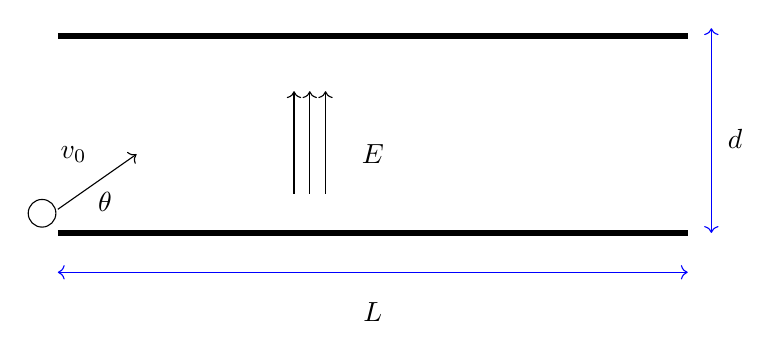
\begin{tikzpicture}
    	\draw [line width=2pt](0,0) -- (8,0);
    	\draw [line width=2pt](0,2.5) -- (8,2.5);
        \draw [->](3,0.5)--(3,1.8);
        \draw [->](3.2,0.5)--(3.2,1.8);
        \draw [->](3.4,0.5)--(3.4,1.8);
        \draw [->](0,0.3)--(1,1);
        \draw (-0.2,0.25) circle [radius=5pt];
        \draw [<->,blue] (0,-0.5)--(8,-0.5);
        \draw [<->,blue] (8.3,0)--(8.3,2.6);
        \node at (4,1) {$E$};
        \node at (0.6,0.4) {$\theta$};
        \node at (0.2,1){$v_0$};
        \node at (4,-1) {$L$};
        \node at (8.6,1.2){$d$};
    \end{tikzpicture}
    \end{center}

    \begin{minipage}{0.6\textwidth}
    \item Suatu bola bermassa $m$ digantungkan dengan sutas tali pada suatu bidang bermuatan yang terdistribusi merata (non-konduktor). Bola bermuatan $q$ dan bola seimbang ketika tali membentuk sudut $\theta$ bidang dengan vertikal. Hitung kerapatan muatan bidang!
    \end{minipage}
    \hfill
    \begin{minipage}{0.25\textwidth}
    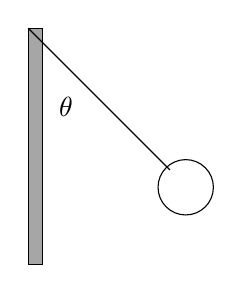
\begin{tikzpicture}
        \filldraw[fill=gray!70] (0,0) rectangle (0.18,3);
        \draw (1.8,1.2)--(0,3);
        \draw (2,0.98) circle [radius=10pt];
        \node at (0.48,2) {$\theta$};
    \end{tikzpicture}
    \end{minipage}

    \item Suatu elektron $115keV$ ditembakkan ke arah suatu lembaran plastik yang mempunyai kerapatan permukaan $-2.08\mu C/m^{2}$. Dari jarak berapa elektron harus ditembakkan agar kecepatan saat menyentuh lembaran itu nol?
\end{enumerate}
\noindent\underline{\textbf{Potensial Listrik}}
\begin{enumerate}
    \item Suatu \textit{Geiger Counter} (alat pencacah partikel) terdiri dari logam berbentuk silinder dengan diameter $2.1cm$. Di sumbu silinder terdapat suatu kawat berdiameter $1.34\times10^{-4}cm$. Jika diantara logam dan kawat diberi tegangan $855V$, hitung besar medan listrik pada permukaan kawat dan permukaan silinder!

    \item Suatu pesawat luar angkasa bergerak melewati sekumpulan gas yang terionisasi pada ionosfer bumi. Potensial pesawat ini berubah $-1$ \textit{Volt} saat ia menempuh satu putaran. Degan menganggap pesawat berbentuk bola berjari-jari $10m$, perkirakan berapa jumlah muatan yang dikumpulkannya!

    \item Suatu tetes air membawa muatan $32.0pC$ mempunyai potensial $512V$ di permukaannya. Hitung jari-jari tetesan ini! Jika dua tetesan yang sejenis dengan jari-jari yang sama dengan tetesan di atas bergabung menjadi satu tetes besar. Hitung potensial pada tetes yang baru!

    \item Suatu gelembung sabun berjari-jari $10cm$ dengan ketebalan $3.3\times 10^{-6}cm$ diberi muatan sampai mencapai potensial sebesar $100V$. Gelembung ini kemudian pecah dan menjadi suatu tetesan berbentuk bola. Hitung potensial tetesan ini!.
\end{enumerate}

%
    

\noindent\underline{\textbf{Kapasitor}}
\begin{enumerate}
    \begin{minipage}{0.55\textwidth}
    \item Suatu kapasitor dibentuk dari dua keping tak sejajar dengan luas keping $A$. Hitung kapasitas kapasitor ini!
    \end{minipage}
    \hfill
    \begin{minipage}{0.3\textwidth}
        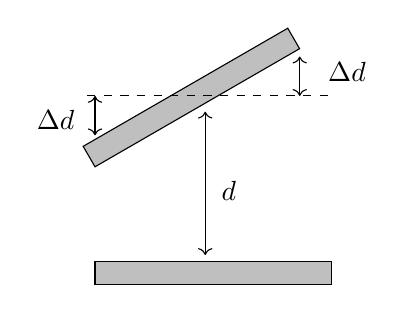
\begin{tikzpicture}
            \filldraw[fill=gray!50,rotate=30] (0,0) rectangle (3,0.3);
            \filldraw[fill=gray!50] (0,-1.2) rectangle (3,-1.5);
            \draw [dashed] (-0.1,0.9)--(3,0.9);
            \draw [<->](1.4,0.7)--(1.4,-1.12);
            \draw [<->] (0,0.4)--(0,0.9);
            \draw [<->] (2.6,0.9)--(2.6,1.4);
            \node at (1.7,-0.3) {$d$};
            \node at (-0.5,0.6){$\Delta d$};
            \node at (3.2,1.2){$\Delta d$};
        \end{tikzpicture}
    \end{minipage}
    \vskip 25pt
     \begin{minipage}{0.45\textwidth}
         \item Hitung kapasitas pengganti antara titik $P$ dan $Q$ dari rangkaian kapasitor berikut!
     \end{minipage}
     \hfill
     \begin{minipage}{0.5\textwidth}
        \begin{circuitikz}
            \draw (0,0) to [short={P},*-] (1,-0.5) to [C={$4\mu F$}] (4,-0.5);
            \draw (1,-0.5) to [short,-] (1,-0.5) to [C={$2\mu F$}] (1,-3);
            \draw (4,-0.5) to [short,-] (4,-0.5) to [C={$8\mu F$}] (4,-3);
            \draw (7,-0.5) to [short,-] (7,-0.5) to [C={$4\mu F$}] (7,-3);
            \draw (4,-0.5) to [short,-] (7,-0.5);
            \draw (1,-3) to [short,-] (4,-3);
            \draw (4,-3) to [C={$2\mu F$}] (7,-3);
            \draw (7,-3) to [short={Q},-*] (8,-3.5);
        \end{circuitikz}
     \end{minipage}

     \item Sekelompok kapasitor dihubungkan seri, lalu paralel. Kapasitas pengganti kapasitor kombinasi paralel 100 kali lebih banyak dibandingkan kombinasi seri. Hitung berapa banyak kapasitor dalam sekelompok ini!
     \vskip 10pt
    \begin{minipage}{0.55\textwidth}
    \item Suatu kapasitor keping sejajar dengan luas permukaan keping $A = 10.5 cm^{2}$ dan jarak antar keping $2d=7.12mm$, ruang antar keping diisi dengan beberapa bahan dielektrik dengan susunan sepeti gambar. Konstanta dielektrik masing-masing bahan dielektrik adalah $\kappa_1 =21, \kappa_2 =42$, dan $\kappa_3=58$
        \begin{enumerate}[a)]
            \item Tentukan kapasitansi kapasitor tersebut
            \item Tentukan muatan dan energi yang tersimpan dalam kapasitor dihubungkan dengan beda potensial $12V$
        \end{enumerate}
    \end{minipage}
    \hfill
    \begin{minipage}{0.35\textwidth}
        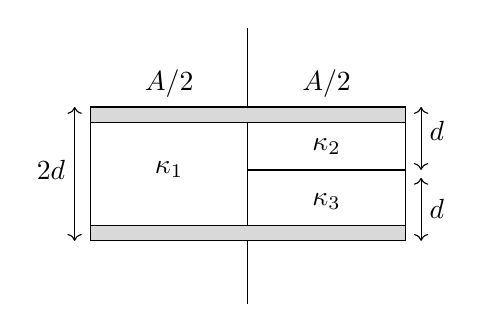
\begin{tikzpicture}
            \draw (0,0)--(0,-1);
            \filldraw [fill=gray!30] (-2,-1) rectangle (2,-1.2);
            \draw (-2,-1.2) rectangle (0,-2.5);
            \draw (0,-1.2) rectangle (2,-1.8);
            \draw (0,-1.8) rectangle (2,-2.5);
            \filldraw[fill=gray!30] (-2,-2.5) rectangle (2,-2.7);
            \draw (0,-2.7) -- (0,-3.5);
            \node at (-1,-0.7){$A/2$};
            \node at (1,-0.7){$A/2$};
            \node at (-1,-1.8){$\kappa_1$};
            \node at (1,-1.5){$\kappa_2$};
            \node at (1,-2.2){$\kappa_3$};
            \draw [<->] (-2.2,-1)--(-2.2,-2.7);
            \draw [<->] (2.2,-1)--(2.2,-1.8);
            \draw [<->] (2.2,-1.9)--(2.2,-2.7);
            \node at (-2.5,-1.8){$2d$};
            \node at (2.4,-1.3){$d$};
            \node at (2.4,-2.3){$d$};
        \end{tikzpicture}
    \end{minipage}
    
     
    \end{enumerate}

\pagebreak
\begin{center}
    \underline{\large \textbf{Pembahasan Latihan Soal Bab 1 dan Bab 2}}
\end{center}
\begin{tabular}{l l}
    Mata Kuliah & : Fisika 2 \\
    Kelas & : 44 \\
    Dosen & : Sefi Novendra Patrialova, S.Si., M.T. \\
    Asisten & : Surya Anoraga Justitia Yusman
\end{tabular}
\vskip10pt
\hrule
\vskip10pt
\noindent\underline{\textbf{Gaya Coulomb}}
\begin{enumerate}
    \item \underline{\textbf{Osilasi Muatan Akibat Muatan Lain}}
    \vskip5pt
    Dua muatan positif $+Q$ ditempatkan pada jarak $b$. Suatu muatan positif $+q$ dan massa $m$ diletakkan di antara kedua muatan ini. Kemudian muatan ini digerakkan sedikit searah dengan garis penghubung kedua muatan, lalu dilepaskan sehingga muatan akan berosilasi. Hitung periode osilasi ini! Hitung juga periode osilasi jika $+q$ diganti dengan $-q$ tetapi digerakkan dalam arah tegak lurus garis penghubung kedua muatan!
    
    a) $+q$ sejajar garis penghubung keuda muatan
    \begin{center}
        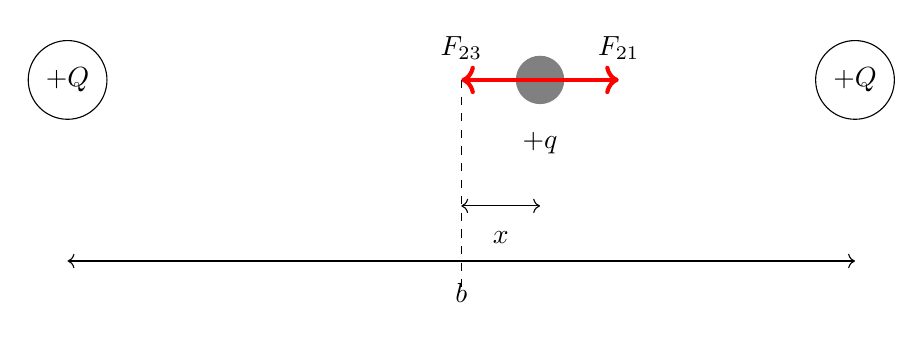
\begin{tikzpicture}
            \draw (-2,0) circle [radius=5mm];
            \filldraw[gray] (4,0) circle [radius=3mm]; 
            \draw (8,0) circle [radius=5mm];
            \node at (-2,0){$+Q$};
            \node at (8,0){$+Q$};
            \node at (4,-0.8){$+q$};
            %\node at (-2,0.8){$q_1$};
            %\node at (4,0.8){$q_2$};
            %\node at (8,0.8){$q_3$};
            \draw [<->] (-2,-2.3)--(8,-2.3);
            \draw [<->] (3,-1.6)--(4,-1.6);
            \node at (3.5,-2){$x$};
            \node at (3,-2.7){$b$};
            \draw[dashed] (3,0)--(3,-2.7);
            \filldraw [line width=1.5pt, red, <-] (3,0)--(4,0);
            \filldraw [line width=1.5pt, red, ->] (4,0)--(5,0);
            \node at (3,0.4){$F_{23}$};
            \node at (5,0.4){$F_{21}$};
        \end{tikzpicture}
    \end{center}

    \begin{minipage}{0.5\textwidth}
    \begin{align*}
    \sum F = ma\\
    -F_{23}+F_{21} = ma\\
    -\frac{kqQ}{(\frac{b}{2}-x)^{2}}+\frac{kqQ}{(\frac{b}{2}+x)^{2}} = ma\\
    -kqQ\left ( \frac{1}{(\frac{b}{2}-x)^{2}}-\frac{1}{(\frac{b}{2}+x)^{2}} \right) = ma\\
    -kqQ\left ( \frac{\left ( \frac{b}{2}+x \right)^{2}-\left ( \frac{b}{2}-x \right )^{2}}{\left ( \frac{b}{2}+x \right)^{2}\left ( \frac{b}{2}-x \right )^{2}} \right ) = ma\\
    -kqQ\left ( \frac{2b}{\left ( \left ( \frac{b}{2} \right )^{2} -x^{2}\right )^{2}} \right )x = ma
    \end{align*}
    Untuk $x$ sangat kecil maka $x^{2} \approx 0$, sehingga
    \end{minipage}
    \hfill
    \begin{minipage}{0.5\textwidth}
    \begin{align*}
    -kqQ\left ( \frac{2b}{\left ( \frac{b}{2} \right )^{4}} \right )x &=ma\\   
    -kqQ\left ( \frac{32}{b^{3}} \right )x &=m\frac{d^{2}x}{dt^{2}}\\ 
    \frac{d^{2}x}{dt^{2}} + \frac{32kqQ}{mb^{3}}x&=0\\
    \omega^{2}=\frac{32kqQ}{mb^{3}} \\
    \omega = \sqrt{\frac{32kqQ}{mb^{3}}} \\
    \frac{2\pi}{T}= \sqrt{\frac{32kqQ}{mb^{3}}} \\
    \fbox{$T = 2\pi\sqrt{\frac{mb^{3}}{32kqQ}}$}
    \end{align*}
    \end{minipage}
    
    \pagebreak
    b) $-q$ tegak lurus garis penghubung keuda muatan

    \begin{center}
        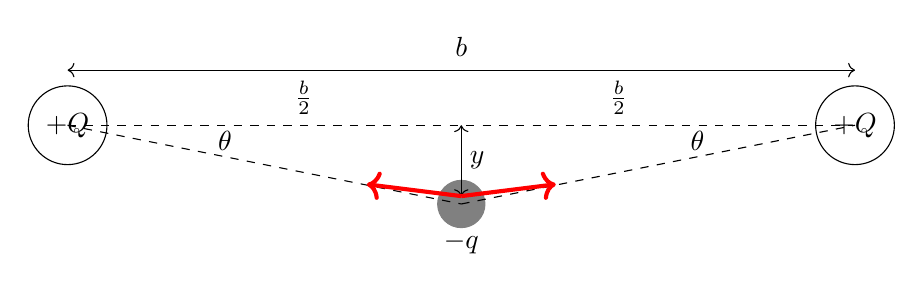
\begin{tikzpicture}
            \draw (-2,0) circle [radius=5mm];
            \filldraw[gray] (3,-1) circle [radius=3mm]; 
            \draw (8,0) circle [radius=5mm];
            \node at (-2,0){$+Q$};
            \node at (8,0){$+Q$};
            \node at (3,-1.5){$-q$};
            %\node at (-2,0.8){$q_1$};
            %\node at (4,0.8){$q_2$};
            %\node at (8,0.8){$q_3$};
            \draw [<->] (-2,0.7)--(8,0.7);
            \draw [<->] (3,0)--(3,-0.9);
            \node at (3.2,-0.45){$y$};
            \node at (3,1){$b$};
            \draw[dashed] (-2,0)--(3,-1);
            \draw[dashed] (3,-1)--(8,0);
            \draw[dashed](-2,0)--(8,0);
            \node at (1,0.35) {$\frac{b}{2}$};
            \node at (5,0.35) {$\frac{b}{2}$};
            \node at (0,-0.2) {$\theta$};
            \node at (6,-0.2) {$\theta$};
            \draw[red,line width=1.5pt,->](3,-0.9)--(1.8,-0.75);
            \draw[red,line width=1.5pt,->](3,-0.9)--(4.2,-0.75);
        \end{tikzpicture}
    \end{center}
    \begin{minipage}{0.5\textwidth}
    Gaya-gaya yang dialami muatan $-q$ pada \\ arah vertikal
    \begin{center}
        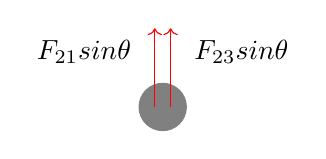
\begin{tikzpicture}
            \filldraw[gray] (0,0) circle [radius=3mm];
            \draw [red,->](-0.1,0)--(-0.1,1);
            \draw [red,->](0.1,0)--(0.1,1);
            \node at (-1,0.7){$F_{21}sin\theta$};
            \node at (1,0.7){$F_{23}sin\theta$};
        \end{tikzpicture}
    \end{center}
    \begin{align*}
    \sum F=ma\\
    -F_{21}sin\theta-F_{23}sin\theta=ma\\
    -\frac{kqQ}{\left ( \frac{b}{2}cos\theta \right )^{2}}sin\theta-\frac{kqQ}{\left ( \frac{b}{2}cos\theta \right )^{2}}sin\theta=ma\\
    -\frac{2kqQ}{\left ( \frac{b}{2}cos\theta \right )^{2}}sin\theta=ma \\    
    \end{align*}
    
    \end{minipage}
    \hfill
    \begin{minipage}{0.4\textwidth}
    Untuk sudut kecil $cos\theta \approx 1$ \\ dan $sin\theta \approx \theta$
    \begin{align*}
    -\frac{2kqQ}{\left ( \frac{b}{2} \right )^{2}}\theta=ma \\
    -\frac{8kqQ}{b^{2}}\theta=ma \\
    -\frac{8kqQ}{b^{2}}\frac{y}{\frac{b}{2}}=m\frac{d^{2}y}{dt^{2}} \\
    \frac{d^{2}y}{dt^{2}}+\frac{16kqQ}{mb^{3}}y=0 \\
    \omega^{2}=\frac{16kqQ}{mb^{3}}\\
    \frac{2\pi}{T}=\sqrt{\frac{16kqQ}{mb^{3}}}\\
    \fbox{$T=2\pi\sqrt{\frac{mb^{3}}{16kqQ}}$}
    \end{align*}
    \end{minipage}
\end{enumerate}

%\pagebreak
\noindent \underline{\textbf{Medan Listrik}}
\vskip 10pt
\begin{enumerate}
    \item \underline{\textbf{Elektron Bergerak Parabola dalam Pengaruh Medan Listrik}}
    \vskip5pt
    Suatu elektron ditembakkan dengan kecepatan awal $v_0$ dan dengan sudut elevasi $\theta$. Jarak kedua keping $d$ dan panjang keping $L$. Jika $v_0 = 5.83\times 10^6 m/s$ dan $\theta = 39^{\circ} ; E= 1870N/C$ (arah keatas), $d=1.97cm$ dan $L=6.20 cm$. Elektron akan menumbuk keping atas atau keping bawah? Dimana?

    \begin{center}
    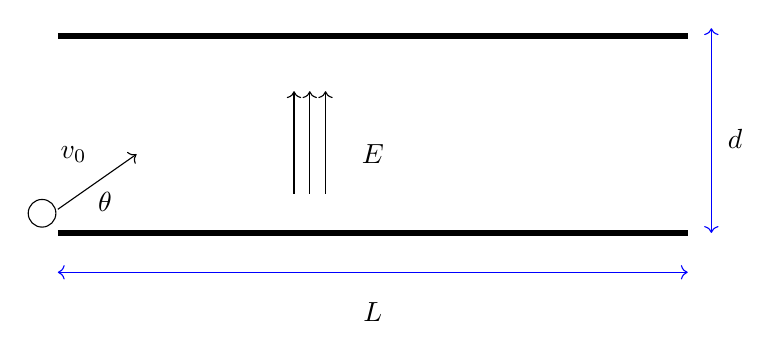
\begin{tikzpicture}
    	\draw [line width=2pt](0,0) -- (8,0);
    	\draw [line width=2pt](0,2.5) -- (8,2.5);
        \draw [->](3,0.5)--(3,1.8);
        \draw [->](3.2,0.5)--(3.2,1.8);
        \draw [->](3.4,0.5)--(3.4,1.8);
        \draw [->](0,0.3)--(1,1);
        \draw (-0.2,0.25) circle [radius=5pt];
        \draw [<->,blue] (0,-0.5)--(8,-0.5);
        \draw [<->,blue] (8.3,0)--(8.3,2.6);
        \node at (4,1) {$E$};
        \node at (0.6,0.4) {$\theta$};
        \node at (0.2,1){$v_0$};
        \node at (4,-1) {$L$};
        \node at (8.6,1.2){$d$};
    \end{tikzpicture}
    \end{center} 
    \pagebreak
    Medan listrik mengarah ke atas maka plat bawah bermuatan positif dan plat atas bermuatan negatif. Elektron akan bergerak parabola dimana selama pergerakannya mengalami percepatan kearah bawah karena elektron akan tertarik menuju plat bawah yang bermuatan positif.\\
    \begin{center}
    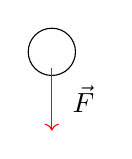
\begin{tikzpicture}
        \draw (0,0) circle [radius=3mm];
        \draw[red,->](0,-0.2)--(0,-1);
        \node at (0.4,-0.6) {$\vec{F}$};
    \end{tikzpicture}
    \end{center}
    Percepatan yang dialami elektron
    \begin{align*}
        \sum \vec{F}=m\vec{a}\\
        q\vec{E}=m\vec{a}\\
        -eE(\hat{i})=m\vec{a}\\
        \vec{a}=-\frac{eE}{m}\hat{i}
    \end{align*}
    Hitung ketinggian maksimum. Jika $y>d$ maka elektron menumbuk plat atas dan sebaliknya jika $y<d$ elektron menumbuk plat bawah.

    Waktu elektron sampai ketinggian maksimum
    \begin{align*}
        v=v_{0y}+at\\
        0=v_{0}sin\theta-\frac{eE}{m}t\\
        t =\frac{m}{eE}v_{0}sin\theta
    \end{align*}

    Ketinggian maksimum
    \begin{align*}
        y&=y_{0}+v_{0y}t+\frac{1}{2}at^{2}\\
        &=y_{0}+v_{0}sin\theta \cdot t-\frac{1}{2}\frac{eE}{m}t^{2}\\
        &=0+v_{0}sin\theta \cdot t-\frac{1}{2}\frac{eE}{m}t^{2}\\
        &=v_{0}sin\theta \left ( \frac{m}{eE}v_{0}sin\theta \right )-\frac{1}{2}\frac{eE}{m}\left ( \frac{m}{eE}v_{0}sin\theta \right )^{2}\\
        &=\left (\frac{m}{eE}v_{0}^{2}sin^{2}\theta\right )-\frac{1}{2}\left ( \frac{m}{eE}v_{0}^{2}sin^{2}\theta \right )\\
        &=\frac{m}{2eE}v_{0}^{2}sin^{2}\theta\\
        &=\frac{9.11\times 10^{-31}}{2\cdot 1.6\times 10^{-19}\cdot 1870}\left ( 5.83\times10^{6} \right )^{2}sin^{2}39^{\circ}\\
        y&=0.0205m\\
        y&=2.05cm
    \end{align*}
        Karena $y>d$ maka elektron menumbuk plat atas. Selanjutnya hitung waktu elektron menumbuk plat atas (pada ketinggian $d$) kemudian dapat dihitung pula jarak tempuh pada arah horizontal.
    \begin{align*}
        y&=y_{0}+v_{0y}t+\frac{1}{2}at^{2}\\
        d&= 0 +v_{0}sin\theta\cdot t-\frac{1}{2}\frac{eE}{m}\cdot t^{2}\\
        1.97\times10^{-2}&=3.66\times 10^{6}\cdot t-1.64\times 10^{14}\cdot t^{2}\\
        &1.64\times 10^{14}\cdot t^{2}-3.66\times 10^{6}\cdot t+1.97\times10^{-2}=0\\
        t&=\frac{-(-3.66\times 10^{6})\pm \sqrt{(-3.66\times 10^{6})^{2}-(4\cdot 1.64\times 10^{14}\cdot 1.97\times10^{-2})}}{2\cdot 1.64\times 10^{14}}\\
        t&=(1.115\times10^{-8})\pm (2.09\times10^{-9})
    \end{align*}
    Karena elektron bergerak parabola, maka elektron (jika tidak ada plat) dapat mencapai ketinggian $d$ sebanyak 2 kali. Karena ada plat atas, maka waktu yang dipilih adalah waktu yang pertama (simbol negatif) sehingga 
    \begin{align*}
        t&=(1.115\times10^{-8})- (2.09\times10^{-9})\\
        t&=9.06\times10^{-9}s
    \end{align*}
    Posisi horizontal elektron menumbuk plat atas
    \begin{align*}
        x&=v_{0x}t\\
        &=v_{0}cos\theta\cdot t\\
        &=(5.83\times 10^{6})cos(39)^{\circ}\cdot 9.06\times10^{-9}\\
        &=0.041m\\
        &\fbox{$x\approx4.1cm$}
    \end{align*}

% == 

    \begin{minipage}{0.6\textwidth}
    \item \underline{\textbf{Kesetimbangan Bandul Bermuatan}}
    \vskip5pt
    Suatu bola bermassa $m$ digantungkan dengan sutas tali pada suatu bidang bermuatan yang terdistribusi merata (non-konduktor). Bola bermuatan $q$ dan bola seimbang ketika tali membentuk sudut $\theta$ bidang dengan vertikal. Hitung kerapatan muatan bidang!
    \end{minipage}
    \hfill
    \begin{minipage}{0.25\textwidth}
    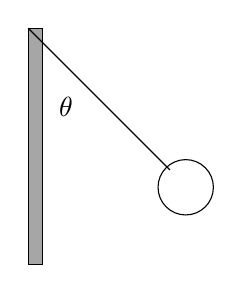
\begin{tikzpicture}
        \filldraw[fill=gray!70] (0,0) rectangle (0.18,3);
        \draw (1.8,1.2)--(0,3);
        \draw (2,0.98) circle [radius=10pt];
        \node at (0.48,2) {$\theta$};
    \end{tikzpicture}
    \end{minipage}

    \begin{center}
    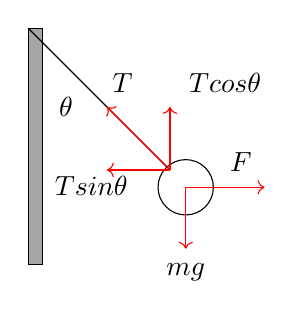
\begin{tikzpicture}
        \filldraw[fill=gray!70] (0,0) rectangle (0.18,3);
        \draw (1.8,1.2)--(0,3);
        \draw (2,0.98) circle [radius=10pt];
        \node at (0.48,2) {$\theta$};
        \draw [red,->] (1.8,1.2)--(1,2);
        \draw [red,->] (1.8,1.2)--(1.8,2);
        \draw [red,->] (1.8,1.2)--(1,1.2);
        \node at (1.2,2.3){$T$};
        \node at (2.5,2.3){$Tcos\theta$};
        \node at (0.8,1){$Tsin\theta$};
        \draw [red,->] (2,0.98)--(2,0.2);
        \node at (2,-0.1){$mg$};
        \draw [red,->] (2,0.98)--(3,0.98);
        \node at (2.7,1.3){$F$};
    \end{tikzpicture}
    \end{center}

    Sistem pada keadaan setimbang
    \vskip5pt
    \begin{minipage}{0.3\textwidth}
    \begin{align*}
        \sum F_{x}&=0\\
        F-Tsin\theta&=0 \\
        F&=Tsin\theta \\
        qE &= Tsin\theta \hskip10pt (1)
    \end{align*}
    \end{minipage}
    \hfill
    \begin{minipage}{0.3\textwidth}
    \begin{align*}
        \sum F_{y}&=0\\
        Tcos\theta-mg&=0\\
        Tcos\theta&=mg \hskip10pt (2)
    \end{align*}
    \end{minipage}
    \hfill
    \begin{minipage}{0.3\textwidth}
    \begin{align*}
        \frac{Tsin\theta}{Tcos\theta}&=\frac{qE}{mg}\\
        tan\theta&=\frac{qE}{mg} \hskip10pt (3)
    \end{align*}
    \end{minipage}
    
    \pagebreak
    \begin{minipage}{0.3\textwidth}
    \vskip5pt
    \begin{center}
    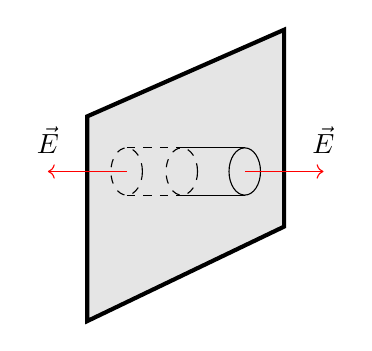
\begin{tikzpicture}
        \filldraw[fill=gray!20,line width=1.5pt] (0,-0.1)--(2.5,1)--(2.5,-1.5)--(0,-2.7)--cycle;
        \draw (2,-0.8) ellipse (0.2 and 0.3);
        \draw [dashed](0.5,-0.8) ellipse (0.2 and 0.3);
        \draw [dashed](1.2,-0.8) ellipse (0.2 and 0.3);
        \draw (1.2,-0.5) -- (2,-0.5);
        \draw (1.2,-1.1) -- (2,-1.1);
        \draw [dashed](0.5,-0.5)--(1.2,-0.5);
        \draw [dashed](0.5,-1.1) -- (1.2,-1.1);
        \draw [red,->](2,-0.8)--(3,-0.8);
        \draw [red,->](0.5,-0.8)--(-0.5,-0.8);
        \node at (3,-0.4){$\vec{E}$};
        \node at (-0.5,-0.4){$\vec{E}$};
    \end{tikzpicture}
    \end{center}
    \end{minipage}
    \hfill
    \begin{minipage}{0.3\textwidth}
    Gunakan Hukum Gauss
    \begin{align*}
        \oint \vec{E}\cdot\vec{dA}&=\frac{q}{\varepsilon_{0}}\\
        2E\cdot A&=\frac{q}{\varepsilon_{0}}\\
        E&=\frac{q}{2A\varepsilon_{0}}\\
        E&=\frac{\sigma}{2\varepsilon_{0}}\hskip10pt (4)
    \end{align*}    
    \end{minipage}
    \hfill
    \begin{minipage}{0.3\textwidth}
    Substitusi $(4)$ ke $(3)$
    \begin{align*}
        tan\theta&=\frac{qE}{mg} \\
        tan\theta&=\frac{q}{mg}\frac{\sigma}{2\varepsilon_{0}}\\
        &\fbox{$\sigma = \frac{2mg\varepsilon_{0}tan\theta}{q}$}
    \end{align*}    
    \end{minipage}

    \item \underline{\textbf{Perlambatan Elektron Oleh Plat Bermuatan}}
    \vskip5pt 
    Suatu elektron $115keV$ ditembakkan ke arah suatu lembaran plastik yang mempunyai kerapatan permukaan $-2.08\mu C/m^{2}$. Dari jarak berapa elektron harus ditembakkan agar kecepatan saat menyentuh lembaran itu nol?

    \begin{minipage}{0.5\textwidth}
    \begin{center}
    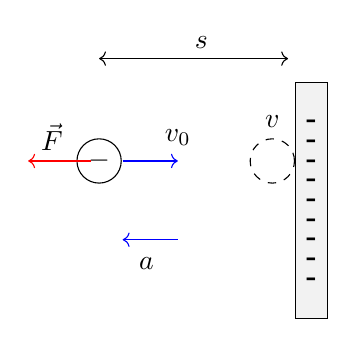
\begin{tikzpicture}
        \draw (0,0) circle [radius=8pt];
        \draw [dashed](2.2,0) circle [radius=8pt];
        \node at (0,0){$-$};
        \filldraw [fill=gray!10] (2.5,1) rectangle (2.9,-2);
        \foreach \x in {1,0.5,...,-3}{
        \node at (2.7,\x*0.5) {\textbf{-}};
        }
        \draw [<->] (0,1.3)--(2.4,1.3);
        \node at (1.3,1.5){$s$};
        \draw [blue,->] (0.3,0)--(1,0);
        \node at (1,0.3){$v_{0}$};
        \node at (2.2,0.5){$v$};
        \draw [blue,<-] (0.3,-1)--(1,-1);
        \node at (0.6,-1.3){$a$};
        \draw [red,->] (-0.1,0)--(-0.9,0);
        \node at (-0.6,0.3){$\vec{F}$};
    \end{tikzpicture}
    \end{center}
    \end{minipage}
    \hfill
    \begin{minipage}{0.4\textwidth}
    \begin{align*}
        E_{k}&=115keV\\
            &= 115(10^{3})(1.6\times10^{-19})\\
            &= 1.84\times 10^{-14}J\\
        \sigma&=-2.08\mu C/m^{2}\\
        &= -2.08\times 10^{-6}C/m^{2}
    \end{align*}
    \end{minipage}
    \vskip5pt
    Elektron (bermuatan negatif) mendekati plat yang memiliki rapat muatan negatif. Karena muatan sejenis (tolak menolak), elektron lama kelamaan akan diperlambat hingga berhenti ketika menyentuh plat. 

    \begin{minipage}{0.4\textwidth}
    \begin{align*}
        \vec{E}&=\frac{\sigma}{2\varepsilon_{0}}\\
        \frac{\vec{F}}{q}&=\frac{\sigma}{2\varepsilon_{0}}\\
        -ma&=\frac{q\sigma}{2\varepsilon_{0}}\\  
    \end{align*}
    \end{minipage}
    \hfill
    \begin{minipage}{0.5\textwidth}
    \begin{align*}
        a&=-\frac{-e\sigma}{2m\varepsilon_{0}}\\
        a&= -\frac{(-1.6\times10^{-19})(-2.08\times 10^{-6})}{2(9.11\times10^{-31})(8.85\times10^{-12})}\\
        a &= -2.06\times10^{16}m/s^{2}
    \end{align*}
    \end{minipage}
    Gunakan persamaan GLBB untuk menghitung jarak elektron ketika mula-mula ditembakkan
    
    \begin{minipage}{0.5\textwidth}
    \begin{align*}
        E_{k}&=\frac{1}{2}mv_{0}^{2}\\
        v_{0}^{2}&=\frac{2E_{k}}{m}\\
        &=\frac{2\cdot1.84\times10^{-14}}{9.11\times10^{-31}}\\
        &= 4.03\times10^{16}(m/s)^{2}
    \end{align*}
    \end{minipage}
    \hfill
    \begin{minipage}{0.5\textwidth}
    \begin{align*}
        v^{2}&=v_{0}^{2}+2as\\
        0 &= (4.03\times10^{16})+2(-2.06\times10^{16})s\\
        s &= \frac{4.03\times10^{16}}{2\cdot2.06\times10^{16}}\\
        s &= 0.978 m\\
        &\fbox{$s = 97.8cm$}
    \end{align*}
    \end{minipage}
    
\end{enumerate}

\pagebreak
\noindent \underline{\textbf{Potensial Listrik}}
\vskip 10pt
\begin{enumerate}
    \item \underline{\textbf{Potensial \textit{Geiger Counter}}}
    \vskip5pt
    Suatu \textit{Geiger Counter} (alat pencacah partikel) terdiri dari logam berbentuk silinder dengan diameter $2.1cm$. Di sumbu silinder terdapat suatu kawat berdiameter $1.34\times10^{-4}cm$. Jika diantara logam dan kawat diberi tegangan $855V$, hitung besar medan listrik pada permukaan kawat dan permukaan silinder!
    \vskip8pt
    \begin{minipage}{0.3\textwidth}
    Muatan yang tersimpan
    \begin{align*}
        V&=-\int_{r_{k}}^{r_{s}}\vec{E}\cdot\vec{dr} \\
        &=-\int_{r_{k}}^{r_{s}}\frac{Q}{2\pi\varepsilon_{0}r}dr \\
        &=-\frac{Q}{2\pi\varepsilon_{0}}ln\left ( \frac{r_{k}}{r_{s}} \right )\\
        V&=\frac{Q}{2\pi\varepsilon_{0}}ln\left ( \frac{r_{s}}{r_{k}} \right )\\
        Q &= \frac{2\pi\varepsilon_{0}V}{ln\left ( \frac{r_{s}}{r_{k}} \right )}\\
        Q &= \frac{855\cdot2\cdot3.14\cdot8.85\times10^{-12}}{ln\left ( \frac{\frac{1}{2}\cdot2.1\times10^{-2}}{\frac{1}{2}\cdot1.34\times10^{-4}\times10^{-2}} \right )}\\
        Q &= 4.91\times10^{-9}C
    \end{align*}
    \end{minipage}
    \hfill
    \begin{minipage}{0.6\textwidth}
    a) Medan listrik pada permukaan silinder
        \begin{align*}
        E&=\frac{Q}{2\pi\varepsilon_{0}r}\\
        E&=\frac{4.91\times10^{-9}}{2\cdot\3.14\cdot8.85\times10^{-12}\cdot\frac{1}{2}\cdot1.34\times10^{-4}\times10^{-2}}\\
        E&=1.32\times10^{8}=132\times10^{6}V/m\\
        &\fbox{$E=132MV/m$}
        \end{align*}
    b) Medan listrik pada permukaan kawat
        \begin{align*}
        E&=\frac{Q}{2\pi\varepsilon_{0}r}\\
        E&=\frac{4.91\times10^{-9}}{2\cdot\3.14\cdot8.85\times10^{-12}\cdot\frac{1}{2}\cdot2.1\times10^{-2}}\\
        E&=8413.7V/m\\
        &\fbox{$E=8.41kV/m$}
        \end{align*}
    \end{minipage}


    \item \underline{\textbf{Muatan Menempel pada Pesawat Luar Angkasa}}
    \vskip5pt
    Suatu pesawat luar angkasa bergerak melewati sekumpulan gas yang terionisasi pada ionosfer bumi. Potensial pesawat ini berubah $-1$ \textit{Volt} saat ia menempuh satu putaran. Degan menganggap pesawat berbentuk bola berjari-jari $10m$, perkirakan berapa jumlah muatan yang dikumpulkannya!
    \vskip8pt
    \begin{minipage}{0.4\textwidth}
    \begin{align*}
        W &= \int\vec{F}\cdot\vec{dr}\\
        \Delta V &= \int\vec{E}\cdot\vec{dr}\\
        &=  \int\frac{kdq}{r}\\
        &= \int_{0}^{2\pi R}\frac{k\lambda}{R}dL\\
        &=\frac{k\lambda}{R}2\pi R\\
    \end{align*}
    \end{minipage}
    \hfill
    \begin{minipage}{0.6\textwidth}
    \begin{align*}
        \Delta V &= \frac{kQ}{R}\\
        -1&=\frac{9\times10^{-9}}{10}Q\\
        Q &= \frac{-10}{9\times10^{-9}}\\
        Q &= -1.11\times10^{-9}C\\
        &\fbox{$Q =-1.11nC$}
    \end{align*}
    \end{minipage}
    \pagebreak
    \item \underline{\textbf{Potensial tetesan air}}
    \vskip5pt
    Suatu tetes air membawa muatan $32.0pC$ mempunyai potensial $512V$ di permukaannya. Hitung jari-jari tetesan ini! Jika dua tetesan yang sejenis dengan jari-jari yang sama dengan tetesan di atas bergabung menjadi satu tetes besar. Hitung potensial pada tetes yang baru!
    \begin{align*}
        V&=\frac{kQ}{R}\\
        R&=\frac{kQ}{V}\\
        &= \frac{9\times10^{9}\cdot32\times10^{-12}}{512}\\
        &=0.000562m\\
        &\fbox{$R=0.562mm$}
    \end{align*}

    Tetesan air bergabung menjadi satu muatan yang lebih bisa. Dengan menganggap rapat muatan mula-mula dan ketika sudah bergabung adalah sama maka
    \begin{minipage}{0.5\textwidth}
    \begin{align*}
        \rho_{awal}=\rho_{baru}\\
        \frac{Q_{awal}}{V_{awal}}=\frac{Q_{baru}}{V_{baru}}\\
        \frac{Q}{\frac{4}{3}\pi R^{3}}=\frac{2Q}{\frac{4}{3}\pi r^{3}}\\
        \frac{Q}{R^{3}}=\frac{2Q}{r^{3}}\\
        r^{3}=2R^{3}\\
        r=2^{\frac{1}{3}}R\\
    \end{align*}
    \end{minipage}
    \hfill
    \begin{minipage}{0.3\textwidth}
    \begin{align*}
        V &= \frac{k(2Q)}{r}\\
        V &= \frac{2\cdot512}{2^{\frac{1}{3}}}\\
        &\fbox{$V= 813V$}
    \end{align*}
    \end{minipage}

    \item \underline{\textbf{Potensial Gelembung Sabun}}
    \vskip5pt
    Suatu gelembung sabun berjari-jari $10cm$ dengan ketebalan $3.3\times 10^{-6}cm$ diberi muatan sampai mencapai potensial sebesar $100V$. Gelembung ini kemudian pecah dan menjadi suatu tetesan berbentuk bola. Hitung potensial tetesan ini!.

    \begin{center}
    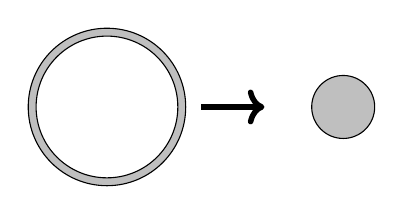
\begin{tikzpicture}
    \filldraw[fill=gray!50] (0,0) circle [radius=1cm];
    \filldraw[fill=white] (0,0) circle [radius=0.9cm];
    \filldraw[fill=gray!50] (3,0) circle [radius=0.4cm];
    \draw [line width=2pt,->](1.2,0)--(2,0);
    \end{tikzpicture}
    \end{center}

    Gelembung (kulit bola) dipecahkan sehingga menjadi tetesan berbentuk bola. Maka muatan gelembung = muatan tetesan dan volume gelembung = volume tetesan.

    \begin{minipage}{0.4\textwidth}
    Volume gelembung (kulit bola) dan Volume tetesan (bola) sama
    \begin{align*}
        v_{gelembung}&=v_{tetesan}\\
        4\pi R^{2}\cdot t &= \frac{4}{3}\pi r^{3}\\
        r^{3}&=3R^{2}t\\
        r&=(3R^{2}t)^{1/3}
    \end{align*}

    \end{minipage}
    \hfill
    \begin{minipage}{0.4\textwidth}
    Potensial gelembung dan tetesan
    \begin{align*}
        V_{gelembung}&=\frac{kQ}{R}\\
        V_{tetesan}&=\frac{kQ}{r}\\
    \end{align*}
    \end{minipage}
    \vskip15pt
    Sehingga potensial dari tetesan
    \begin{align*}
        V_{gelembung}R &= V_{tetesan}r\\
        V_{tetesan}&=\frac{R}{r}V_{gelembung}\\
        &=\frac{R}{(3R^{2}t)^{1/3}}V_{gelembung}\\
        &=\frac{10\times10^{-2}}{(3\cdot (10\times10^{-2})^{2}(3.3\times10^{-6}\times10^{-2}))^{1/3}}100\\
        &=10033.55\\
        &\fbox{V\approx 10kV}
    \end{align*}
\end{enumerate}

\end{document}